\documentclass[11 pt,letterpaper,titlepage]{article} %TITLEPAGE ARGUMENT
\usepackage{graphicx,float}
\usepackage[section]{placeins}
\usepackage[margin=1in]{geometry}
\usepackage[colorlinks=true,allcolors=black]{hyperref}
\usepackage[toc,page]{appendix}
\usepackage{listings}


\title{\LARGE \bf
    BIF705 Lab 3: Clustering in R
    }
\author{Christopher Eeles}
\date{\small \today}

\begin{document}

% TITLE PAGE
\maketitle

% TABLE OF CONENTS
\tableofcontents

%\newpage

% ENUMERATE
\section{Enumerate}
    \begin{enumerate}
        \item Item 1
        \item Item 2
        \item Item 3
    \end{enumerate}

\section{Introduction}

    Leveraging R packages to facilitate biological data analysis and visualization is an essential skill for bioinformatics professionals.
    Such packages enable simple implementation of mathematically and/or computationally complex data analysis methodologies by those lacking the time or technical expertise to write algorithms themselves.
    In doing so, they allow researchers to focus on making the greatest possible impact in their field of study, without the need to spend time and resources learning the intricacies of cutting edge data analytics techniques.
    This report will focus on the application of the \texttt{multtest}, \texttt{spls}, \texttt{gplots} and \texttt{dextend} R packages to the analysis and visualization of differential gene expression data from several classes of B-cell lymphomas.$^2$
    

    The lymphoma dataset generated by Alizadeh \textit{et al.} (2000) will be imported from \texttt{spls} and processed to be a suitable input for generating a red/green heat map of the sample expression data.$^1$
    Hierarchical clustering will be conducted using Euclidean distance metrics for the complete, single, and average linkage algorithms, with each visualized using a dendrogram.
    The data will then be alternatively clustered using the k-means algorithm at three iteration levels with results displayed in confusion matrices for each respective clustering.$^1$
    Results will be compared to known classifications of B-cell lymphomas from Alizadeh's study to assess the accuracy of different parameters for the hierarchical and k-means clustering algorithms for grouping differential gene expression data.

% SECTION
\section{Results}
    % SUBSECTION
    \subsection{Heatmap}

    % FIGURES
    \begin{figure}[H]
        \centering
        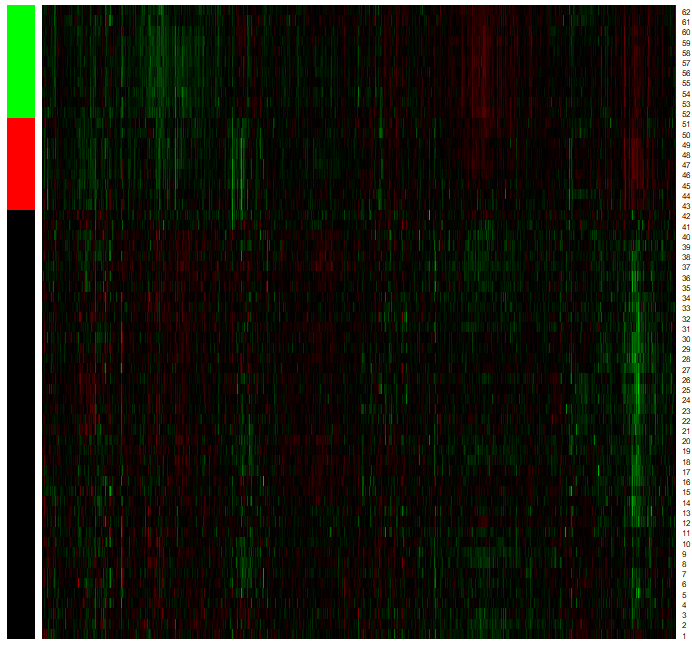
\includegraphics[width=4in]{Figures/heatmap.png}
        \caption{Red-green Heatmap of B-cell Lymphoma Data}
        \label{fig:heatmap}
    \end{figure}

    \subsection{Dendrograms}
    \begin{figure}[H]
        \centering
        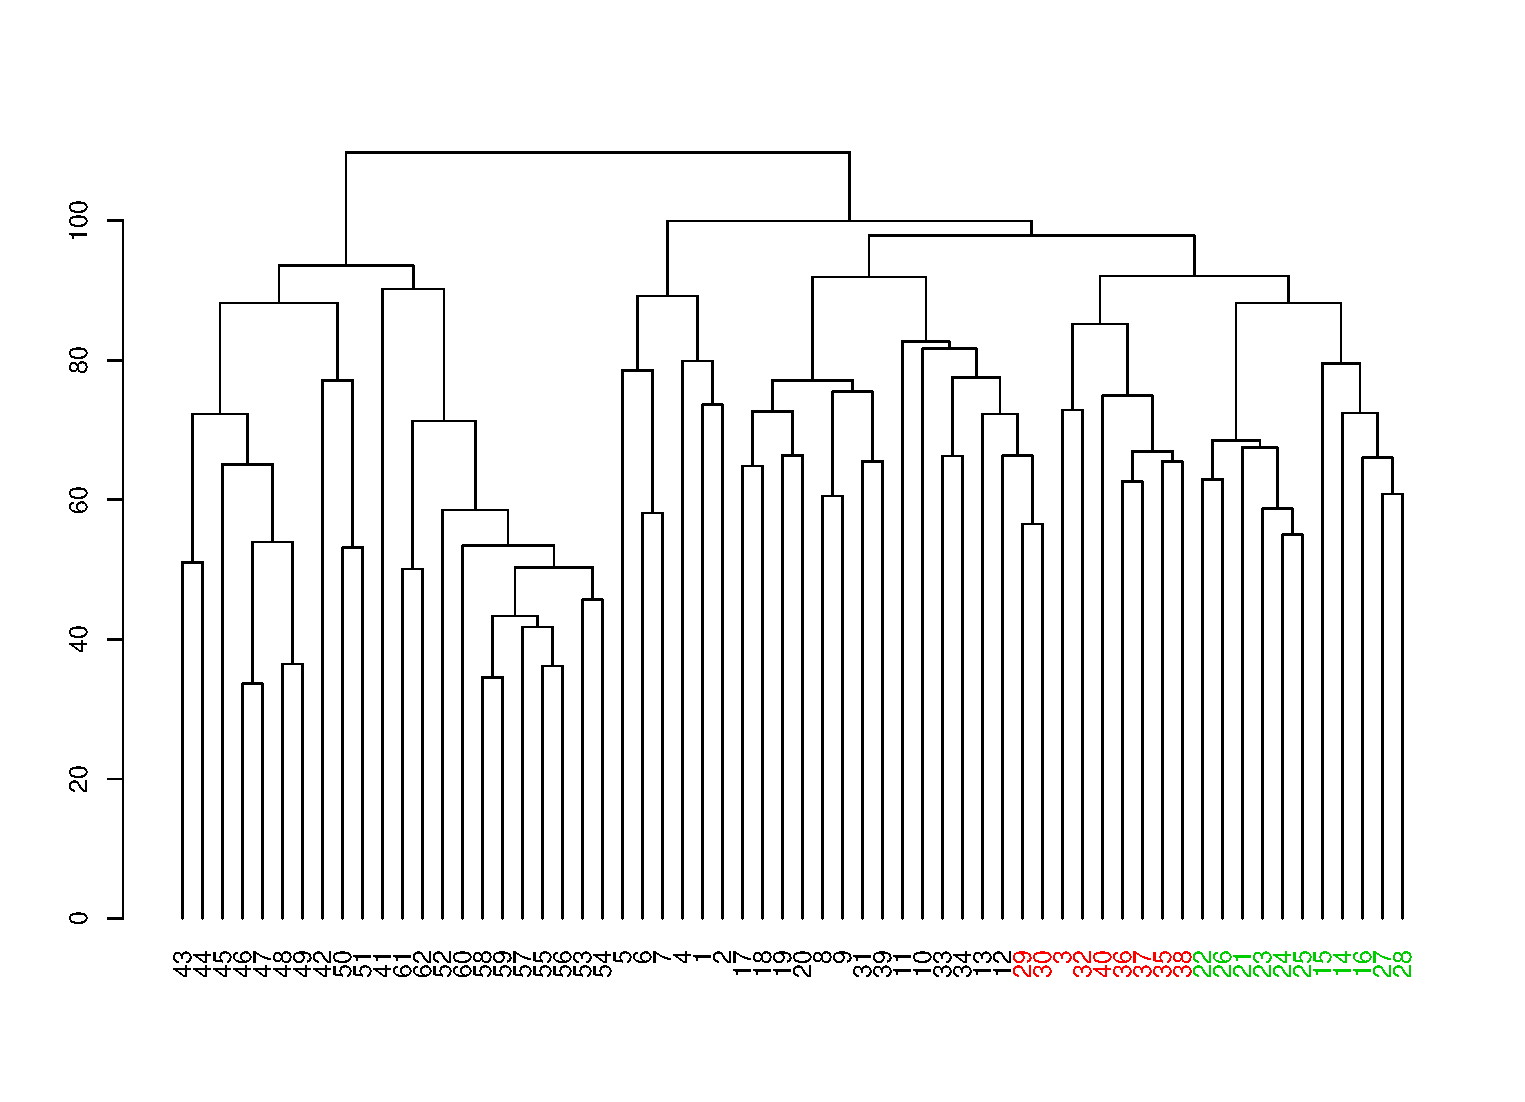
\includegraphics[width=5in]{Figures/dendComplete.pdf}
        \caption{Dendrogram of Hierarchical Clustering with Complete Linkage Algorithm}
        \label{fig:dend1}
    \end{figure}

    \begin{figure}[H]
        \centering
        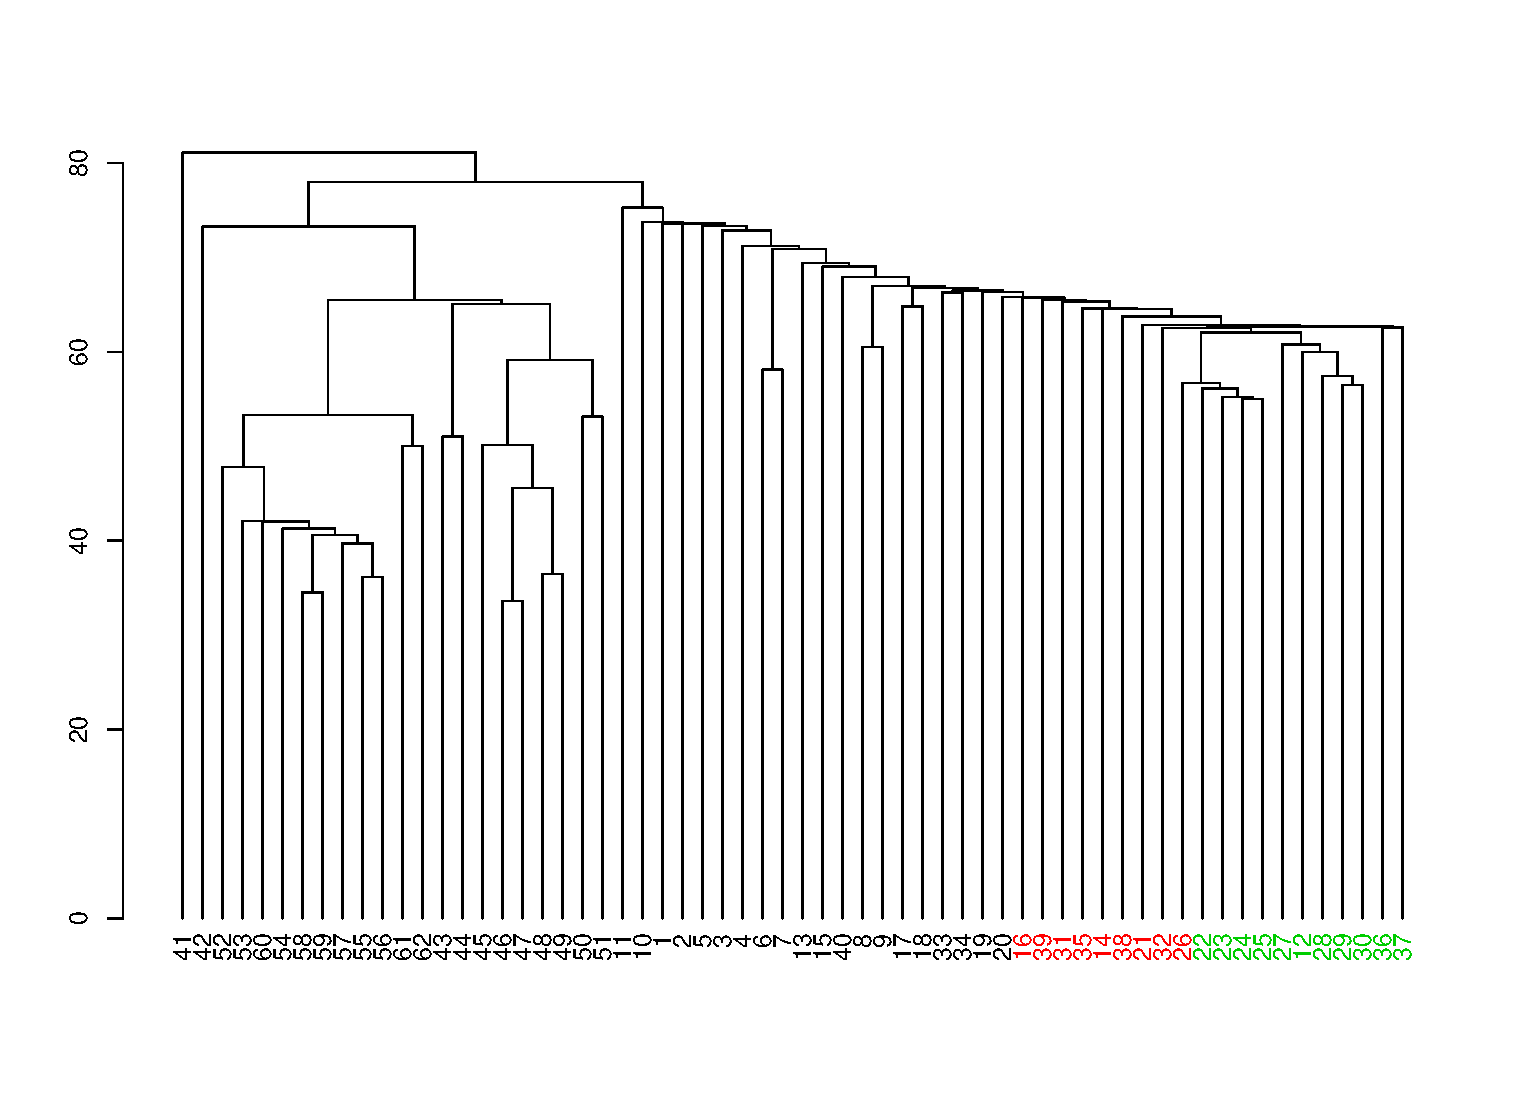
\includegraphics[width=5in]{Figures/dendSingle.pdf}
        \caption{Dendrogram of Hierarchical Clustering with Single Linkage Algorithm}
        \label{fig:dend2}
    \end{figure}

    \begin{figure}[H]
        \centering
        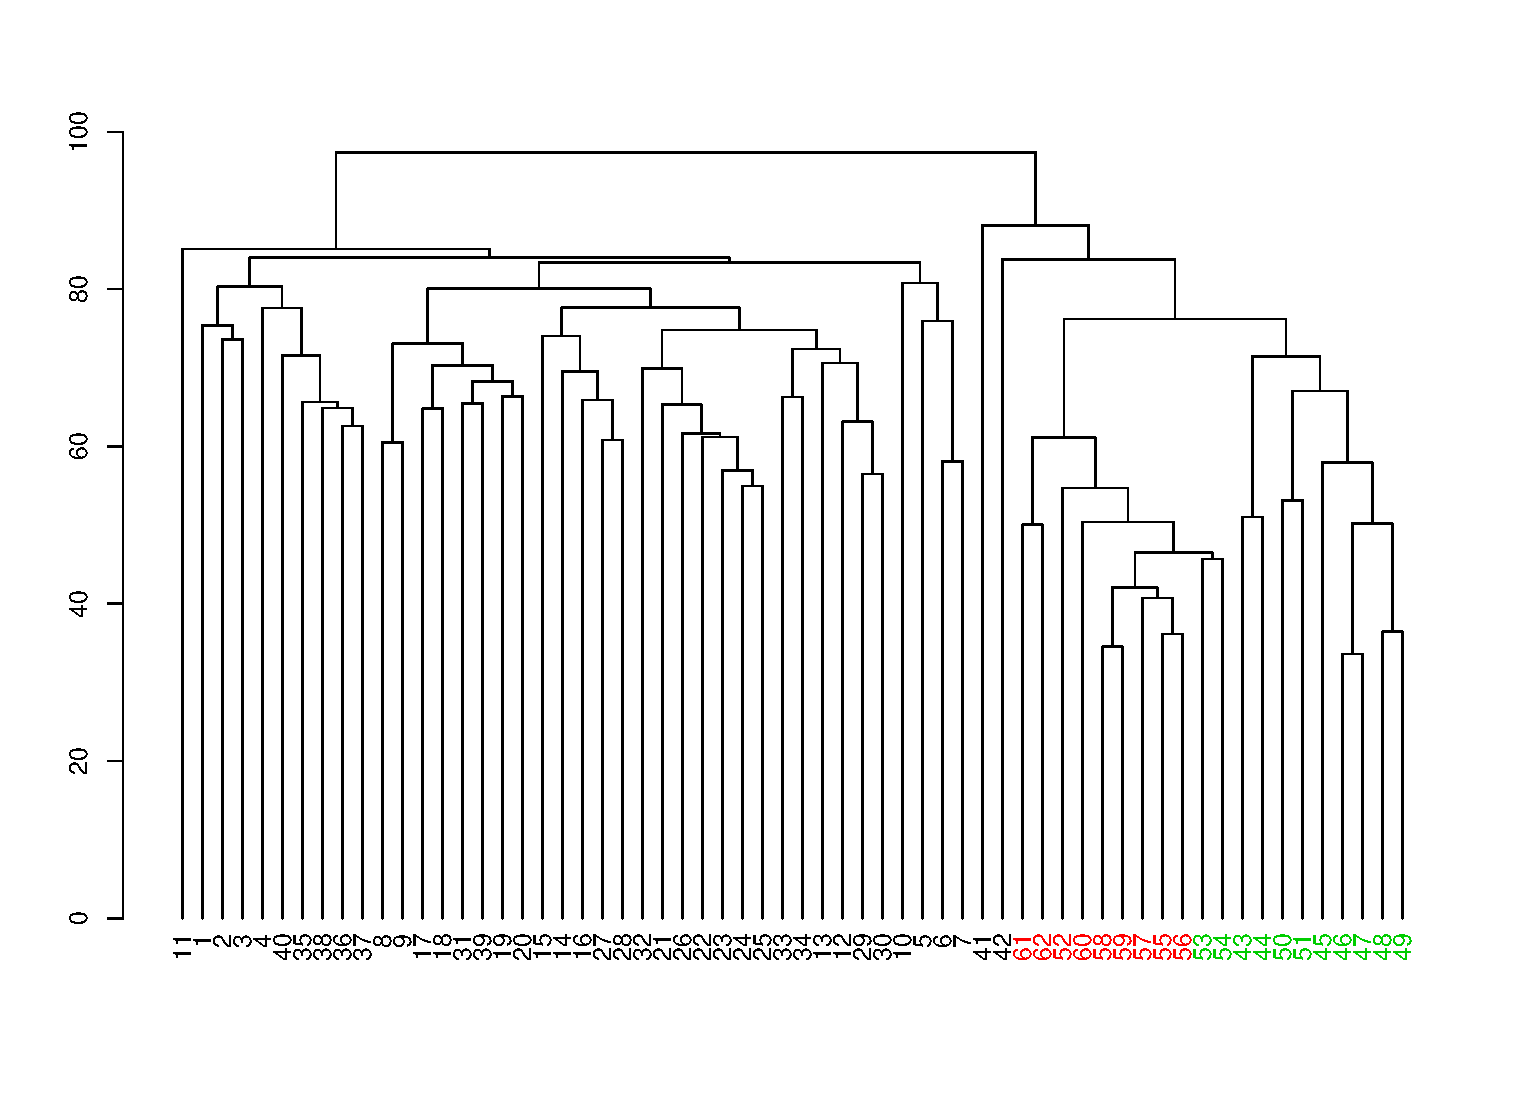
\includegraphics[width=5in]{Figures/dendAverage.pdf}
        \caption{Dendrogram of Hierarchical Clustering with Average Linkage Algorithm}
        \label{fig:dend3}
    \end{figure}

    \subsection{K-means}

    \begin{figure}[H]
        \centering
        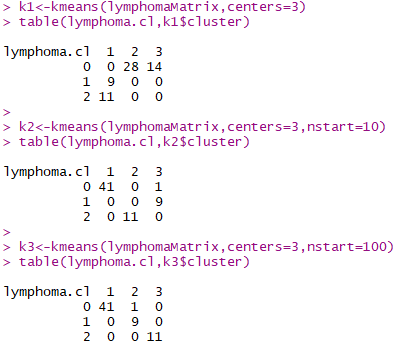
\includegraphics[width=2in]{Figures/kmeans.png}
        \caption{K-means Confusion Matrices for Default, 10 and 100 Iterations}
        \label{fig:kmeans}
    \end{figure}

\section{Discussion and Conclusion}

    Figure 1 shows the heat map plotted using R, with the three major cell types of B-cell lymphoma represented by the colour bar on the left.
    Based on the results of the Aldizeh study, correct clustering would place samples 1 through 42 into the first group ("black"), samples 43 through 51 in the second group ("green") and samples 52 through 62 in the third group ("red).
    Examining the dendrogram from the complete linkage hierarchical clustering (hclust) in Figure 2, it is clear that the colourations do not map correctly to the groupings from the experimental data. 
    On closer inspection, colouration of the sample numbers appear to map only to position in the graph, therefore bearing no relation to either the true or estimated sample clusters; this may be due to an experimental error in the syntax of dendrogram plotting. 
    This fact---combined with the lack of discernible significance of the colour groupings to the biological interpretation of this data---is deemed to justify exclusion of these groupings from further discussion.

    The top right branch of Figure 2 encompasses a large number of samples and maps well to group one from the experimental data, with a noted misclassification of sample 42. The left branch breaks down into two larger subgrouping which also map reasonably to the experimental data. The left subgrouping approximates the true membership of group two with the exclusion of sample 42 and the right subgrouping corresponds to the third experimentally determined cluster with 41 as an outlier. Given these results the complete linkage algorithm appears to be a reasonable method for predicting clusters for the B-cell lymphoma data, with less than five errors.

    The single linkage hclust algorithm in Figure 3 also does a reasonable job predicting the high level categorization of the B-cell lymphoma data, though it performs notably worse than the complete linkage algorithm. 41 is again an outlier, this time excluded as distinct from the other groupings on the leftmost branch. Ignoring this branch, the rightmost group maps well to the first cluster from the experimental data, with the inclusion of less than five outlier. If 42 is excluded as an outlier the subsequent branches correlate closely with cluster two and three, respectively, from the experimental data. Overall, these predictions are still reasonably accurate, including less than ten outliers compared to the true classifications.

    The average linkage algorithm in Figure 4 performed intermediate to the the previous two hclust methods. The rightmost branch approximates the true clustering of group one. The leftmost branch, if 41 and 42 are excluded as outliers, maps well to the true clustering of group three on the right and group two on the left. While this dendrogram also includes less than five outliers, the miscategorization of samples 41 and 42 constitute a decrease in accuracy when compared to the complete linkage algorithm of Figure 1.
    Therefore the most accurate hierarchical clustering algorithm in the context of the B-cell lymphoma data is the complete linkage.


    For the confusion matrices calculated using iterative K-means clustering, approximation with default settings performed extremely poorly compared to the hclust algorithms. When increasing iterations to ten, the predictions for cluster one (zero in the matrix) become reasonable with 41 out of 42 samples correctly sorted. The remaining two clusters were were completely incorrect, though it grouped the correct number of observations into each predicted group, inverting clusters two and tree compared to the true groupings. K-means with 100 iterations performed better than all of the hclust algorithms with only one miscategorization for cluster one. Based on these observations, k-means is a more accurate method of clustering than the hierarchical algorithm with Euclidean distances, at least if more iterations are possible.

    Overall these results validate all four algorithms as reasonable predictors of groupings for the B-cell lymphocyte data presented in the Alizadeh study. Further tweaking of parameters could result in even better predictions and therefore further study of the parameters available in the R packages utilized in this study may allow more confident prediction in the future. While these methods have proven reasonably accurate, gaining a deeper understanding of the algorithms behind these R tools and their respective parameters could enable more accurate and therefore impactful analysis of differential gene expression data. 

% BIBLIOGRAPHY
\begin{thebibliography}{1}

    \bibitem{1} School of Biological Sciences and Applied Chemistry. (2019). BIF701 Topic 3: Clustering. Seneca College: Toronto, ON.

    \bibitem{2} Aldizeh, A.A., \textit{et al}. (2000). Distinct types of diffuse large B-cell lymphoma identified by gene expression profiling. \textit{Nature 403} (pp. 503–551)  DOI: \url{https://doi.org/10.1038/35000501}

    \bibitem{3} Liaw, A., Gentleman, R., Maechler, M. and Hubert, W. (N.d.). Draw a Heat Map. R Documentation. Retrieved from \url{https://stat.ethz.ch/R-manual/R-devel/library/stats/html/heatmap.html}

\end{thebibliography}

\appendix
\section{R Script}
\begin{lstlisting}[breaklines=T,numbers=left,numberstyle=\tiny]{R}
library(BiocManager)
library(affy)
library(affydata)
library(multtest)
library(spls)
library(gplots)
library(dendextend)
# stats is a base package in R, don't need to load it.

#### Data Processing

# Import data set
data(lymphoma)

# Converting list to matrix and storing class vector

lymphomaDF <- as.data.frame(lymphoma)

lymphomaMatrix <- as.matrix(lymphomaDF)

lymphoma.cl <- lymphoma[["y"]] # Classes are DLBCL, FL and CLL lymphocyte malignancies

lymphomaCL <- lymphoma.cl + 1 # Added one because zero doesn't represent a colour

lymphomaColor <- c(rep("black",42),rep("red",9),rep("green",11))

#### Heat Map

# Generate heatmap of data using red/green colour mapping
heatmap(lymphomaMatrix,Colv=NA,Rowv=NA,col=redgreen(75),labCol="",RowSideColors=lymphomaColor)

#### Euclidean Linkage

# Complete linkage with Euclidean

hc1<-hclust(dist(lymphomaMatrix))
dend1<-as.dendrogram(hc1)
dend1<-color_labels(dend1,col=lymphomaCL)
eucComplete<-list(plot(dend1))

# Single linkage with Euclidean

hc2<-hclust(dist(lymphomaMatrix),method='single')
dend2<-as.dendrogram(hc2)
dend2<-color_labels(dend2,col=lymphomaCL)
eucSingle<-list(plot(dend2))

# Average linkage with Euclidean

hc3<-hclust(dist(lymphomaMatrix),method='average')
dend3<-as.dendrogram(hc3)
dend3<-color_labels(dend3,col=lymphomaCL)
eucAverage<-list(plot(dend3))

#### K-means Clustering

k1<-kmeans(lymphomaMatrix,centers=3)
        table(lymphoma.cl,k1$cluster)

k2<-kmeans(lymphomaMatrix,centers=3,nstart=10)
table(lymphoma.cl,k2$cluster)

k3<-kmeans(lymphomaMatrix,centers=3,nstart=100)
table(lymphoma.cl,k3$cluster)
\end{lstlisting}

\end{document}